\documentclass{article}
\usepackage{graphicx} % Required for inserting images
\usepackage{indentfirst}

% Set page size and margins
% Replace `letterpaper' with `a4paper' for UK/EU standard size
\usepackage[letterpaper,top=2cm,bottom=2cm,left=3cm,right=3cm,marginparwidth=1.75cm]{geometry}

\title{Tema 1 - Algoritmica Grafurilor}

\author{Mihail Popovici, Luca Petrovici, Alexandru-Constantin Iov, George-Razvan Rusu}
\begin{document}
\maketitle

\section*{\fontsize{20}{50}\selectfont Problema 1}
{\fontsize{14}{16}\selectfont  Un graf eulerian este un graf în care există un parcurs închis care trece prin toate muchiile sale. Deoarece graful $G = (V,E)$ este conex și toate nodurile sale au gradul par, acesta este un graf eulerian. 
\par O metodă de a înlocui fiecare muchie a lui $G$ cu exact un arc astfel încât în noul digraf $G'$ fiecare nod să aibă gradul interior egal cu cel exterior este de a trece prin parcurs. Prin schimbarea, înspre sensul de mers, a fiecărei muchii cu un arc, de fiecare dată când trecem printr-un nod îi vom crește atât gradul interior cât și cel exterior cu 1. Singura excepție este primul nod din parcurs, al cărui grad exterior vă fi incrementat cu 1 la începutul parcurgerii, rămânând diferit de cel interior până la finalizarea parcurgerii, când vor fi egalate.
}

\section*{\fontsize{20}{50}\selectfont Problema 2}
\subsection*{\fontsize{16}{30}\selectfont Subpunctul a}
{\fontsize{14}{16}\selectfont  Presupunem prin reducere la absurd ca $xy \in E \setminus  E'$ și $x$ nu este strămoș al lui $y$ sau invers.
\par Din aceasta, rezultă că $x$ și $y$ au un strămoș comun în arborele generat de parcurgerea $DFS$. Dacă $x$ și $y$ au strămoș comun în arborele $DFS$ înseamnă că parcurgerea a trecut prin $x$ și a rămas fară noduri de explorat. Apoi, acesta s-a întors înapoi la strămoșul comun și a continuat parcurgerea din acesta, urmând să treacă prin y. 
\par Însă, pentru ca $DFS$-ul să ajungă înapoi la strămoșul comun, atunci ar trebui ca $x$ să nu mai aibă niciun vecin neexplorat, dar deoarece $xy \in$ E, algoritmul nu ar mai fi ajuns la acel strămoș comun, plasandu-l pe $y$ ca fiul lui $x$ , adică $x$ este strămoșul lui $y$ .
\par Deoarece am ajuns la contradicție, înseamnă că presupunerea este falsă, deci dacă $xy \in E \setminus E'$, $x$ este un ascendent al lui $y$ sau invers.
}

\subsection*{\fontsize{16}{30}\selectfont Subpunctul b}
{\fontsize{14}{16}\selectfont
Presupunem prin reducere la absurd ca $\exists u$ a.i. $up_d(u) > level(u)$. 
\par Asa cum am demonstrat la subpunctul a, dacă 2 noduri sunt vecine în graful inițial, atunci unul dintre ele va fi stramoșul celuilalt, adică va avea nivelul mai mic ca celălalt.  În cel mai rău caz, $up_d(u)$ va fi format din toți strămoșii lui u, adică $uv \in E \setminus E', \forall v \in N_g(u)$. În acest caz, $up_d(u) = level(u)$, ceea ce înseamna că $up_d(u)$ nu poate fi mai mare decat $level(u)$, deci presupunerea este eronată.
\par Rezultă că $up_d(u) \le level(u), \forall u \in V$. 
}

\subsection*{\fontsize{16}{30}\selectfont Subpunctul c}
{\fontsize{14}{16}\selectfont
$\forall xy \in E$, aceasta va contribui fie la $up_d(x)$, fie la $up_d(y)$.
\par Muchia nu poate contribui la ambele în același timp, deoarece ar implica $level(x) < level(y)$ și $level(y) < level(x)$ simultan, ceea ce nu este posibil. 
\par În același timp, muchia $xy$ nu poate să nu incrementeze niciun $up_d()$, deoarece ar trebui ca $level(x) < level(y)$ și $level(y) < level(x)$ să fie false în același timp, deci, $level(x) \ge level(y)$ și $level(y) \ge level(x)$ în același timp, adică $level(x) = level(y)$, ceea ce este imposibil deoarece muchia $xy \in E$, rezultă fie $x$ este strămoșul lui $y$, fie $y$ este strămoșul lui $x$ (conform subpunctului a).
\par Așadar, fiecare muchie contribuie la suma de $up_d()$ cu 1, adică în final $\sum_{u \in V} {up}_d(u)
 = m$.
}

\subsection*{\fontsize{16}{30}\selectfont Subpunctul d}
{\fontsize{14}{16}\selectfont
Așa cum am demonstrat la subpunctul b, $up_d(u) \le level(u), \forall u \in V$. Însumând inegalitatea pentru fiecare u, vom obține: \\
 \centerline {$\sum_{u \in V} {up}_d(u) \le \sum_{u \in V} {level(u)}$ } \\
 \par Conform subpunctului c, $\sum_{u \in V} {up}_d(u) = m \Rightarrow m \le \sum_{u \in V} {level(u)}$ , dar $\sum_{u \in V} {level(u)} \le n \cdot level(x)$, unde $x$ este nodul cu cel mai mare level, adică nodul care dă adancimea arborelui $DFS$. Rezultă $m \le n \cdot level(x) \Rightarrow m/n \le level(s)$, adică adancimea lui $T$ este cel puțin $m/n$; 
}

\subsection*{\fontsize{16}{30}\selectfont Subpunctul e}
{\fontsize{14}{16}\selectfont
Fie $G$, graful din figura \ref{fig:graf} și $T$, arborele din figura \ref{fig:arbore}. Pentru a forma în arborele $T$ circuitul $1 \rightarrow 2 \rightarrow 5 \rightarrow 1$ din $G$, ar trebui să introducem atât muchia $1 \rightarrow 5$, cât și $2 \rightarrow 5$. Însa, conform enunțului, $C_{xy}$ reprezintă arborele $T$, la care se adaugă o singură muchie din $G$. Astfel, am găsit un contraexemplu în care nu putem forma toate circuitele din $G$ adăugând doar câte o muchie, rezultând ca afirmația este falsă. În plus, deoarece $\lbrace C_{xy} : xy \in E \backslash E' \rbrace$ nu conține toate circuitele din $G$, atunci nu vom fi niciodată siguri că circuitul de lungime minimă se poate afla prin prelucrarea unei traversări $DFS$ a lui $G$.
}

\begin{figure}[h]
    \centering
    \begin{minipage}{0.45\textwidth}
        \centering
        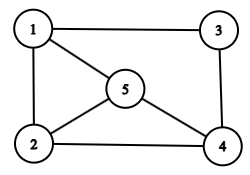
\includegraphics[width=\textwidth]{images/graph_cropped.png}
        \caption{Un graf $G$}
        \label{fig:graf}
    \end{minipage}\hfill
    \begin{minipage}{0.45\textwidth}
        \centering
        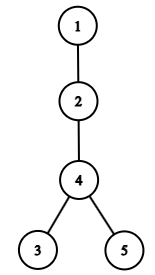
\includegraphics[width=\textwidth]{images/DFS_tree_cropped.png}
        \caption{Arborele traversării $DFS$, pornind din nodul 1}
        \label{fig:arbore}
    \end{minipage}
\end{figure}

\section*{\fontsize{20}{50}\selectfont Problema 3}
\subsection*{\fontsize{16}{30}\selectfont Subpunctul a}
{\fontsize{14}{16}\selectfont
Înainte de a incepe demonstrațiile de la următoarele subpuncte, vom explica întregul algoritm.

În primul for al algoritmului, cozile de arce sunt inițializate cu null.
Apoi, nodul $s$ de start este plasat în mulțimea $S$ a nodurilor vizitate, iar costul drumului minim și nodul anterior al sau sunt actualizate. Ultima instrucțiune din $for$ plasează toate muchiile care ies din $s$ în coada aferentă prețului său.

Apoi, $while$-ul parcurge nodurile grafului până când toate sunt vizitate. Înainte de a incepe prelucrarea, funcția $Search()$ va fi apelată, funcție care va returna muchia corespunzătoare celui mai scurt drum de la origine pana la capătul drept al muchiei. Apoi, capatul drept al muchiei returnate este marcat ca vizitat, îi este actualizat drumul minim și îi este actualizat nodul anterior. 

În final, algoritmul iterează prin toate arcele care ies din $j^*$ și le plasează în coada corespunzatoare.
}
\subsubsection*{\fontsize{14}{20}\selectfont Subpunctul a1}
{\fontsize{14}{16}\selectfont
Este evident că algoritmul va plasa nodurile în $S$ în ordinea crescătoare a costurilor minime a drumurilor din $s$, deoarece atunci când alege o muchie pe care să își continue execuția, compară costurile drumurilor din $s$ până în capătul drept al muchiei, urmând să îl returneze pe cel mai mic. Deoarece nu există costuri negative în digraf, drumurile create cu muchiile din cozi vor continua să crească în cost, deci nu va aparea în cozi niciodată o muchie cu un drum cu cost mai mic decât orice alt drum parcurs în trecut.
}

\subsubsection*{\fontsize{14}{20}\selectfont Subpunctul a2}
{\fontsize{14}{16}\selectfont

Deoarece algoritmul adaugă arce în $L_h$ pe masură ce exploreaza nodurile, iar nodurile sunt alese în ordine crescătoare a costurilor $u_i$, dacă $u_i < u_j$ atunci algoritmul a explorat nodul $i$ înainte de nodul $j$ și, implicit, a adaugat arcele ce ies din $i$ (printre care si $ij$) înaintea celor care ies din $i'$ (printre care si $i'j'$). Astfel, dacă două arce $ij$ și $i'j'$ aparțin aceleiași cozi și $u_i < u_j$, $ij$ apare înaintea lui $i'j'$ in $L_h$.

}

\subsubsection*{\fontsize{14}{20}\selectfont Subpunctul a3}
{\fontsize{14}{16}\selectfont
Luând condițiile în ordine, putem demonstra de ce structura cozii $L_h$ rămâne aceeași pe toată durata algoritmului.
$\lbrace i \in S \rbrace$ : Atunci când adăugam arce în coada $L_h$, iterăm prin vecinii lui $j^*$ și punem în coadă arcele corespunzătoare nodurilor neexplorate. Deoarece adăugarea arcelor în coadă se face dupa ce $j^*$ este marcat ca un nod vizitat, iar nodurile nu sunt scoase niciodată din mulțimea nodurilor vizitate, această condiție este îndeplinită.

$\lbrace$ j $\notin$ S $\rbrace$ : Înainte de apelarea funcției $Search()$, condiția este îndeplinită deoarece adăugăm în cozi doar nodurile care $\notin S$. În timpul apelării, dacă căpatul drept al oricărui arc dintr-o coadă este vizitat, atunci acesta este eliminat din coadă. Astfel, după apelare nu va mai exista în coadă niciun arc cu capătul drept explorat, respectandu-se condiția.

$a_{ij} = \gamma_h$ : Această condiție este permanent îndeplinită pentru că, înainte de a adauga un arc în coadă este verificată.

Astfel, deoarece toate cele 3 condiții sunt îndeplinite, putem spune că $\lbrace ij : i \in S, j \notin S, a_{ij} = \gamma_h \rbrace \subseteq L_h$ înainte și după fiecare iterație a buclei $while$.

}

\subsubsection*{\fontsize{14}{20}\selectfont Subpunctul a4}
{\fontsize{14}{16}\selectfont

La început, cozile $L_h$ sunt inițializate cu valori nule și se adaugă doar muchiile vecine nodului de start. Este important de observat că în această fază doar nodul de start se află în mulțimea $S$ a nodurilor vizitate. După intrarea în bucla while, variabila $ij^*$ primește rezultatul funcției $Search()$, care caută în toate muchiile din $L_h$ și returnează muchia $xy$ aferenta drumului cu cost minim, unde $x \in S$ și $y \notin S$. Abia după ce $ij^*$ este selectat, nodul $j^*$ este adăugat în $S$, iar muchiile incidente cu acesta sunt adăugate în $L_h$, fără ca celelalte capete ale acestor muchii să fie incluse în $S$. Deci, oricum am alege muchia $ij^*$, aceasta va reprezenta drumul cu cel mai mic cost dintre toate celelalte drumuri pe care le putem forma cu muchiile din cozi.

}

\subsection*{\fontsize{16}{30}\selectfont Subpunctul b}
{\fontsize{14}{16}\selectfont
Primul $for$ al algoritmului are o complexitate $O(p)$. Următorul $for$, care itereaza prin vecinii lui $i$ se face in timp constant. $while$-ul principal va itera prin toate nodurile digrafului, adică va avea complexitatea $O(n)$, și va apela funcția $Search()$ la fiecare pas.

Functia $Search()$ verifică fiecare arc din cozi. În cel mai rău caz, va verifica toate arcele la fiecare apelare, adică va avea complexitatea $O(m)$.

În final, complexitatea algoritmului va fi \\
\centerline {$O(p) + O(n) \cdot O(m) = O(n \cdot m)$.}
}

\section*{\fontsize{20}{50}\selectfont Problema 4}

\subsection*{\fontsize{16}{30}\selectfont Subpunctul a}
{\fontsize{14}{16}\selectfont
\par $G'$ este obținut prin eliminarea de muchii din $G$, pe baza unei condiții descrise în algoritmul dat, iar $G$ nu are circuite de lungime $\le 4$. Așadar, $G'$ nu poate avea nici el circuite de lungime $\le 4$ întrucât eliminarea de muchii nu poate genera circuite, ci poate doar menține sau micșora numărul de circuite din acel graf.}

\subsection*{\fontsize{16}{30}\selectfont Subpunctul b}
{\fontsize{14}{16}\selectfont
\par Presupunem prin reducere la absurd că $V_{u,1} \cap V_{u,2} \neq \emptyset$. Înseamna că $\exists x$ astfel încât $x \in V_{u,1}$ și $x \in V_{u,2}$. Pentru că $x \in V_{u,2}$, trebuie să existe $v \in V_{u,1}, v \ne x$ astfel încât $v$ și $x$ să fie adiacente. Dar pentru că $x,v \in V_{u,1}$, înseamnă că $u$ este adiacent cu $x$ și $v$. Astfel, se formează un circuit de lungime 3 ($u \rightarrow v \rightarrow x$), ceea ce contrazice faptul că $G'$ nu conține circuite de lungime $\le 4$. Deci, $V_{u,1} \cap V_{u,2} = \emptyset$.}

{\fontsize{14}{16}\selectfont
\par Dacă oricare două noduri din $V_{u,1}$ sunt adiacente, se formează un circuit de lungime 3, deoarece $u$ este adiacent cu fiecare dintre nodurile din $V_{u,1}$, inclusiv cele două. Acest lucru nu este posibil deoarece $G$ și $G'$ nu conțin circuite de lungime $\le 4$.}

\subsection*{\fontsize{16}{30}\selectfont Subpunctul c}
{\fontsize{14}{16}\selectfont
\par În urma rulării algoritmului, vom obține un graf $G'$ care va avea $n'$ noduri și $m'$ muchii $(n' \le n, m' \le m)$. Așadar, \\
\\ \centerline {$\sum_{u \in G'} {d}_{G'}(u) \ge n' \cdot \frac{m}{n} \Leftrightarrow$}
\\ \centerline {$2 \cdot m' \ge n' \cdot \frac{m}{n} \Leftrightarrow$}
\\ \centerline {$m \le 2 \cdot n \cdot \frac{m'}{n'}$}
Deci, $m = O(n \cdot \frac{m'}{n'})$
}

\end{document}